\documentclass[journal,12pt,twocolumn]{IEEEtran}
\usepackage{setspace}
\usepackage{gensymb}
\singlespacing
\usepackage[cmex10]{amsmath}
\usepackage{amsthm}
\usepackage{mathrsfs}
\usepackage{txfonts}
\usepackage{stfloats}
\usepackage{bm}
\usepackage{cite}
\usepackage{cases}
\usepackage{subfig}
\usepackage{longtable}
\usepackage{multirow}
\usepackage{enumitem}
\usepackage{mathtools}
\usepackage{steinmetz}
\usepackage{tikz}
\usepackage{circuitikz}
\usepackage{verbatim}
\usepackage{tfrupee}
\usepackage[breaklinks=true]{hyperref}
\usepackage{tkz-euclide}
\usetikzlibrary{calc,math}
\usepackage{listings}
    \usepackage{color}                                            %%
    \usepackage{array}                                            %%
    \usepackage{longtable}                                        %%
    \usepackage{calc}                                             %%
    \usepackage{multirow}                                         %%
    \usepackage{hhline}                                           %%
    \usepackage{ifthen}                                           %%
  %optionally (for landscape tables embedded in another document): %%
    \usepackage{lscape}     
\usepackage{multicol}
\usepackage{chngcntr}
\DeclareMathOperator*{\Res}{Res}
\renewcommand\thesection{\arabic{section}}
\renewcommand\thesubsection{\thesection.\arabic{subsection}}
\renewcommand\thesubsubsection{\thesubsection.\arabic{subsubsection}}

\renewcommand\thesectiondis{\arabic{section}}
\renewcommand\thesubsectiondis{\thesectiondis.\arabic{subsection}}
\renewcommand\thesubsubsectiondis{\thesubsectiondis.\arabic{subsubsection}}

% correct bad hyphenation here
\hyphenation{op-tical net-works semi-conduc-tor}
\def\inputGnumericTable{}                                 %%

\lstset{
frame=single, 
breaklines=true,
columns=fullflexible
}

\begin{document}


\newtheorem{theorem}{Theorem}[section]
\newtheorem{problem}{Problem}
\newtheorem{proposition}{Proposition}[section]
\newtheorem{lemma}{Lemma}[section]
\newtheorem{corollary}[theorem]{Corollary}
\newtheorem{example}{Example}[section]
\newtheorem{definition}[problem]{Definition}
\newcommand{\BEQA}{\begin{eqnarray}}
\newcommand{\EEQA}{\end{eqnarray}}
\newcommand{\define}{\stackrel{\triangle}{=}}

\bibliographystyle{IEEEtran}
\providecommand{\mbf}{\mathbf}
\providecommand{\pr}[1]{\ensuremath{\Pr\left(#1\right)}}
\providecommand{\qfunc}[1]{\ensuremath{Q\left(#1\right)}}
\providecommand{\sbrak}[1]{\ensuremath{{}\left[#1\right]}}
\providecommand{\lsbrak}[1]{\ensuremath{{}\left[#1\right.}}
\providecommand{\rsbrak}[1]{\ensuremath{{}\left.#1\right]}}
\providecommand{\brak}[1]{\ensuremath{\left(#1\right)}}
\providecommand{\lbrak}[1]{\ensuremath{\left(#1\right.}}
\providecommand{\rbrak}[1]{\ensuremath{\left.#1\right)}}
\providecommand{\cbrak}[1]{\ensuremath{\left\{#1\right\}}}
\providecommand{\lcbrak}[1]{\ensuremath{\left\{#1\right.}}
\providecommand{\rcbrak}[1]{\ensuremath{\left.#1\right\}}}
\theoremstyle{remark}
\newtheorem{rem}{Remark}
\newcommand{\sgn}{\mathop{\mathrm{sgn}}}
\providecommand{\abs}[1]{\left\vert#1\right\vert}
\providecommand{\res}[1]{\Res\displaylimits_{#1}} 
\providecommand{\norm}[1]{\left\lVert#1\right\rVert}
\providecommand{\mtx}[1]{\mathbf{#1}}
\providecommand{\mean}[1]{E\left[ #1 \right]}
\providecommand{\fourier}{\overset{\mathcal{F}}{ \rightleftharpoons}}
\providecommand{\system}{\overset{\mathcal{H}}{ \longleftrightarrow}}
\newcommand{\solution}{\noindent \textbf{Solution: }}
\newcommand{\cosec}{\,\text{cosec}\,}
\providecommand{\dec}[2]{\ensuremath{\overset{#1}{\underset{#2}{\gtrless}}}}
\newcommand{\myvec}[1]{\ensuremath{\begin{pmatrix}#1\end{pmatrix}}}
\newcommand{\mydet}[1]{\ensuremath{\begin{vmatrix}#1\end{vmatrix}}}
\numberwithin{equation}{subsection}
\makeatletter
\@addtoreset{figure}{problem}
\makeatother

\let\StandardTheFigure\thefigure
\let\vec\mathbf
\renewcommand{\thefigure}{\theproblem}



\def\putbox#1#2#3{\makebox[0in][l]{\makebox[#1][l]{}\raisebox{\baselineskip}[0in][0in]{\raisebox{#2}[0in][0in]{#3}}}}
     \def\rightbox#1{\makebox[0in][r]{#1}}
     \def\centbox#1{\makebox[0in]{#1}}
     \def\topbox#1{\raisebox{-\baselineskip}[0in][0in]{#1}}
     \def\midbox#1{\raisebox{-0.5\baselineskip}[0in][0in]{#1}}

\vspace{3cm}


\title{Assignment 1}
\author{Jaswanth Chowdary Madala}





% make the title area
\maketitle

\newpage

%\tableofcontents

\bigskip

\renewcommand{\thefigure}{\theenumi}
\renewcommand{\thetable}{\theenumi}


\begin{enumerate}
\item If circles are drawn taking two sides of a triangle as diameters, prove that the point of intersection of these circles lie on the third side.
\begin{figure}[ht]
\centering
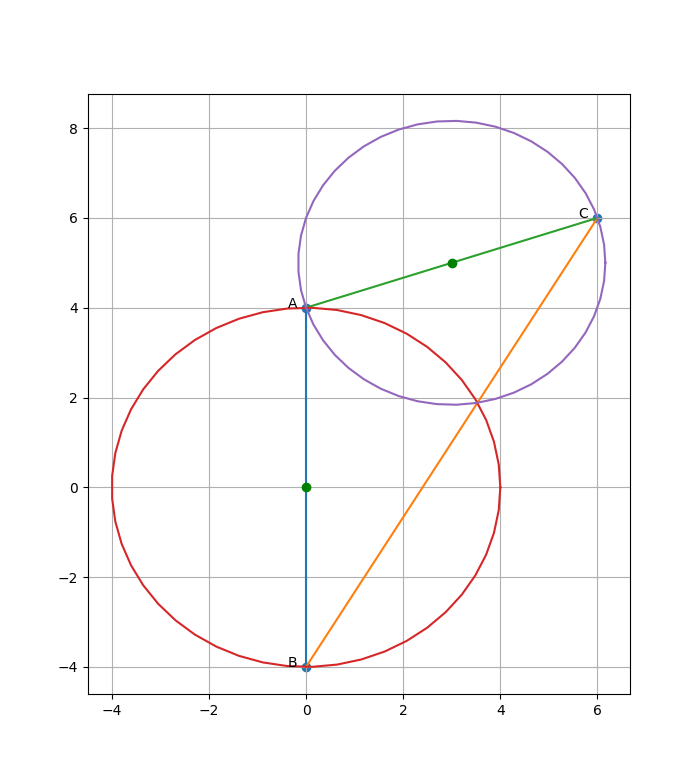
\includegraphics[width = \columnwidth]{figs/fig.png}
\caption{Graph}
\label{fig:1}
\end{figure}

\textbf{Solution:}
Let the traingle be $ABC$, Points $\vec{A},\vec{B},\vec{C}$ are given by,
\begin{align}
\vec{A} = \myvec{0\\4}, \,\vec{B} = \myvec{0\\-4}, \,\vec{C} = \myvec{6\\6}
\end{align}
The equation of circle taking $\vec{AB}$ as diameter is given by,
\begin{align}
\norm{\vec{x}}^2 + 2\vec{u_1}^\top\vec{x} + f_1 &= 0 \\
\vec{u_1} &= -\brak{\frac{\vec{A}+\vec{B}}{2}}\\
&= \myvec{0\\0}\\
r_1 &= \frac{\norm{\vec{AB}}}{2}\\
&= 4\\
f_1 &= \norm{\vec{u_1}}^2 - r_1^2\\
&= -4\\
\norm{\vec{x}}^2 -16 &= 0
\label{eq:1}
\end{align}
The equation of circle taking $\vec{AC}$ as diameter is given by,
\begin{align}
\norm{\vec{x}}^2 + 2\vec{u_2}^\top\vec{x} + f_2 &= 0 \\
\vec{u_2} &= -\brak{\frac{\vec{A}+\vec{C}}{2}}\\
&= -\myvec{3\\5}\\
r_2 &= \frac{\norm{\vec{AC}}}{2}\\
&= \sqrt{10}\\
f_2 &= \norm{\vec{u_2}}^2 - r_2^2\\
&= 24\\
\norm{\vec{x}}^2 -2\myvec{3&5}\vec{x}+24 &= 0
\label{eq:2}
\end{align}
Let the other point of intersection of circles \eqref{eq:1} and \eqref{eq:2} be point $\vec{P}$. The equation of the common chord of intersection of two circles, $AP$ is given by,
\begin{align}
\vec{u_1}^\top\vec{x}-\vec{u_2}^\top\vec{x}+f_1 - f_2 &= 0\\
2\myvec{3 & 5}\vec{x}-16-24&= 0\\
\myvec{3&5}\vec{x} &= 20
\label{eq:3}
\end{align}
The equation \eqref{eq:3} can be written in parametric form as,
\begin{align}
\vec{h} = \myvec{0\\4}, \, \vec{m} = \myvec{-5\\3}\\
\vec{x} = \myvec{0\\4} + \mu \myvec{-5\\3}
\end{align}
The parameter $\mu$ of the points of intersection of line \eqref{eq:4} with the conic section \eqref{eq:5}
\begin{align}
\vec{x} &= \vec{h} + \mu \vec{m}
\label{eq:4}\\
\text{g}\brak{\vec{x}} &= \vec{x}^{\top}\vec{V}\vec{x}+2\vec{u}^{\top}\vec{x}+f=0
\label{eq:5}
\end{align}
is given by the equation 
\begin{align}
\mu^2\vec{m}^{\top}\vec{V}\vec{m} + 2 \mu\vec{m}^{\top}\brak{\vec{V}\vec{h}+\vec{u}} + \text{g}\brak{\vec{h}} &=0
\label{eq:6}
\end{align}
The points of intersection of the circle \eqref{eq:1} and line \eqref{eq:3} are the points $\vec{A}, \vec{P}$. Here we have,
\begin{align}
\vec{V} = \vec{I}, \, \vec{u} &= \vec{O}, \, f = 16\\
\vec{h} = \myvec{0\\4}, \, \vec{m} &= \myvec{-5\\3}\\
\vec{m}^{\top}\vec{V}\vec{m} &= 34\\
\vec{m}^{\top}\brak{\vec{V}\vec{h}+\vec{u}} &= 12\\
\text{g}\brak{\vec{h}} &= 0\\
34\mu^2 + 24 \mu &= 0\\
\mu &= 0, -\frac{12}{17}
\end{align}
$\mu = 0$ corresponds to point $\vec{A}$.
\begin{align}
\vec{P} &= \myvec{0\\4} -\frac{12}{17} \myvec{-5\\3}\\
\vec{P} &= \myvec{\frac{60}{17}\\\\\frac{32}{17}}
\end{align}
The equation of the the line $\vec{BC}$ is given by,
\begin{align}
\vec{m} &= \vec{C}-\vec{B}\\
&= \myvec{6\\10}\\
&= \myvec{3\\5}\\
\vec{n} &= \myvec{-5\\5}\\
\vec{n}^\top\vec{x} &= \vec{n}^\top\vec{B}
\end{align}
\begin{align}
\myvec{-5&3}\vec{x} &= \myvec{-5&3}\myvec{0\\-4}\\
\myvec{-5&3}\vec{x} &= -12
\label{eq:7}\\
\myvec{-5&3}\myvec{\frac{60}{17}\\\\\frac{32}{17}} &= -12
\end{align}
It is clear that the point $\vec{P}$ satisfies the equation of line $\vec{BC}$ \eqref{eq:7}. Hence, the point of intersection of the circles drawn by taking two sides of a triangle as diameters lies on the third side.

The parameters used in the construction are shown in the below table \ref{tab:1}

\begin{table}[h]
\centering
%%%%%%%%%%%%%%%%%%%%%%%%%%%%%%%%%%%%%%%%%%%%%%%%%%%%%%%%%%%%%%%%%%%%%%
%%                                                                  %%
%%  This is a LaTeX2e table fragment exported from Gnumeric.        %%
%%                                                                  %%
%%%%%%%%%%%%%%%%%%%%%%%%%%%%%%%%%%%%%%%%%%%%%%%%%%%%%%%%%%%%%%%%%%%%%%
\begin{center}
\begin{tabular}{|c|c|c|}
\hline
\textbf{Parameter}	&\textbf{Description}& \textbf{Value}\\ \hline
$\vec{A}	$ & vertex of the triangle &	$\myvec{0\\4}$ 	\\ \hline
$\vec{B}	$ & vertex of the triangle &	$\myvec{0\\-4}$	\\ \hline
$\vec{C}$ &vertex of the triangle  &	$\myvec{6\\6}$\\ \hline
\end{tabular}
\end{center}
\caption{}
\label{tab:1}
\end{table}
\end{enumerate}
\end{document}